\section{寄存器描述}
\regover{
{\hyperref[ir-irrx-config]{irrx\_config}}&
\\
\hline
{\hyperref[ir-irrx-int-sts]{irrx\_int\_sts}}&
\\
\hline
{\hyperref[ir-irrx-pw-config]{irrx\_pw\_config}}&
\\
\hline
{\hyperref[ir-irrx-data-count]{irrx\_data\_count}}&
\\
\hline
{\hyperref[ir-irrx-data-word0]{irrx\_data\_word0}}&
\\
\hline
{\hyperref[ir-irrx-data-word1]{irrx\_data\_word1}}&
\\
\hline
{\hyperref[ir-ir-fifo-config-0]{ir\_fifo\_config\_0}}&
\\
\hline
{\hyperref[ir-ir-fifo-config-1]{ir\_fifo\_config\_1}}&
\\
\hline
{\hyperref[ir-ir-fifo-rdata]{ir\_fifo\_rdata}}&
\\
\hline
}

\subsection{irrx\_config}
\label{ir-irrx-config}
地址:0x40010240
 \begin{figure}[H]
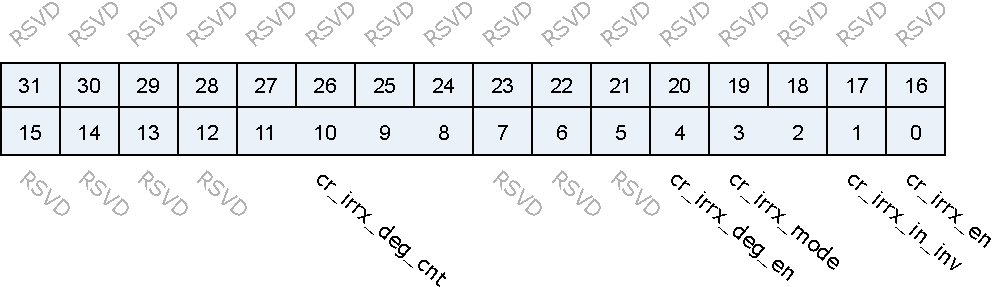
\includegraphics{ir_irrx_config.pdf}
\end{figure}

\regdes{31:12&RSVD& & & \\\hline
11:8&cr\_irrx\_deg\_cnt&r/w&4'd0&De-glitch function cycle count\\\hline
7:5&RSVD& & & \\\hline
4&cr\_irrx\_deg\_en&r/w&1'b0&Enable signal of IRRX input de-glitch function\\\hline
3:2&cr\_irrx\_mode&r/w&2'd0&IRRX mode \par 0: NEC \par 1: RC5 \par 2: SW pulse-width detection mode (SWM) \par 3: Reserved
\\\hline
1&cr\_irrx\_in\_inv&r/w&1'b1&Input inverse signal\\\hline
0&cr\_irrx\_en&r/w&1'b0&Enable signal of IRRX function \par Asserting this bit will trigger the transaction, and should be de-asserted after finish
\\\hline

}
\subsection{irrx\_int\_sts}
\label{ir-irrx-int-sts}
地址:0x40010244
 \begin{figure}[H]
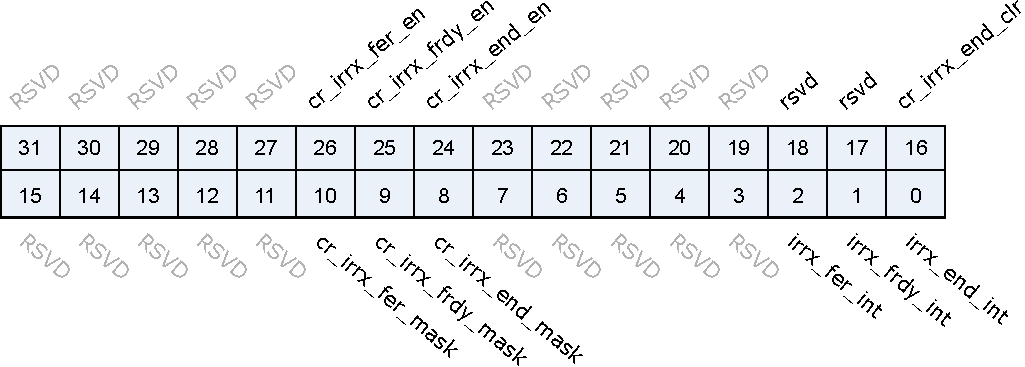
\includegraphics{ir_irrx_int_sts.pdf}
\end{figure}

\regdes{31:27&RSVD& & & \\\hline
26&cr\_irrx\_fer\_en&r/w&1'b1&Interrupt enable of irrx\_fer\_int\\\hline
25&cr\_irrx\_frdy\_en&r/w&1'b1&Interrupt enable of irrx\_frdy\_int\\\hline
24&cr\_irrx\_end\_en&r/w&1'b1&Interrupt enable of irrx\_end\_int\\\hline
23:19&RSVD& & & \\\hline
18&rsvd&rsvd&1'b0&\\\hline
17&rsvd&rsvd&1'b0&\\\hline
16&cr\_irrx\_end\_clr&w1c&1'b0&Interrupt clear of irrx\_end\_int\\\hline
15:11&RSVD& & & \\\hline
10&cr\_irrx\_fer\_mask&r/w&1'b1&Interrupt mask of irrx\_fer\_int\\\hline
9&cr\_irrx\_frdy\_mask&r/w&1'b1&Interrupt mask of irrx\_frdy\_int\\\hline
8&cr\_irrx\_end\_mask&r/w&1'b1&Interrupt mask of irrx\_end\_int\\\hline
7:3&RSVD& & & \\\hline
2&irrx\_fer\_int&r&1'b0&IRRX FIFO error interrupt, auto-cleared when FIFO overflow/underflow error flag is cleared\\\hline
1&irrx\_frdy\_int&r&1'b0&IRRX FIFO ready (rx\_fifo\_cnt > rx\_fifo\_th) interrupt, auto-cleared when data is popped\\\hline
0&irrx\_end\_int&r&1'b0&IRRX transfer end interrupt\\\hline

}
\subsection{irrx\_pw\_config}
\label{ir-irrx-pw-config}
地址:0x40010248
 \begin{figure}[H]
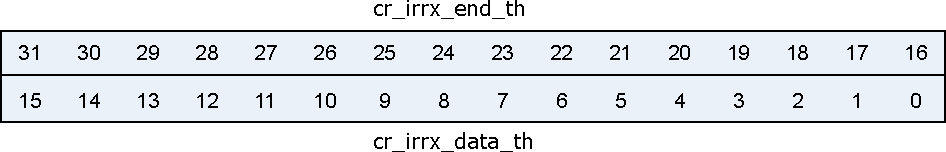
\includegraphics{ir_irrx_pw_config.pdf}
\end{figure}

\regdes{31:16&cr\_irrx\_end\_th&r/w&16'd8999&Pulse width threshold to trigger END condition\\\hline
15:0&cr\_irrx\_data\_th&r/w&16'd3399&Pulse width threshold for Logic0/1 detection (Don't care if SWM is enabled)\\\hline

}
\subsection{irrx\_data\_count}
\label{ir-irrx-data-count}
地址:0x40010250
 \begin{figure}[H]
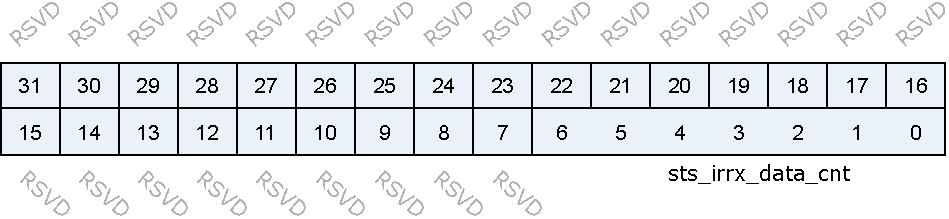
\includegraphics{ir_irrx_data_count.pdf}
\end{figure}

\regdes{31:7&RSVD& & & \\\hline
6:0&sts\_irrx\_data\_cnt&r&7'd0&RX data bit count (pulse-width count for SWM)\\\hline

}
\subsection{irrx\_data\_word0}
\label{ir-irrx-data-word0}
地址:0x40010254
 \begin{figure}[H]
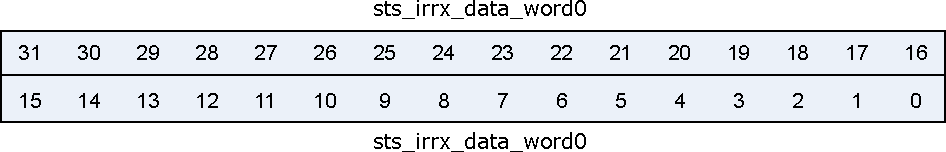
\includegraphics{ir_irrx_data_word0.pdf}
\end{figure}

\regdes{31:0&sts\_irrx\_data\_word0&r&32'h0&RX data word 0\\\hline

}
\subsection{irrx\_data\_word1}
\label{ir-irrx-data-word1}
地址:0x40010258
 \begin{figure}[H]
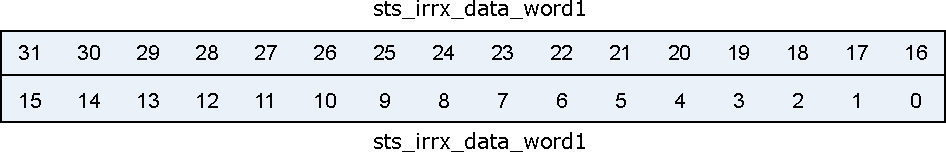
\includegraphics{ir_irrx_data_word1.pdf}
\end{figure}

\regdes{31:0&sts\_irrx\_data\_word1&r&32'h0&RX data word 1\\\hline

}
\subsection{ir\_fifo\_config\_0}
\label{ir-ir-fifo-config-0}
Address:0x40010280
 \begin{figure}[H]
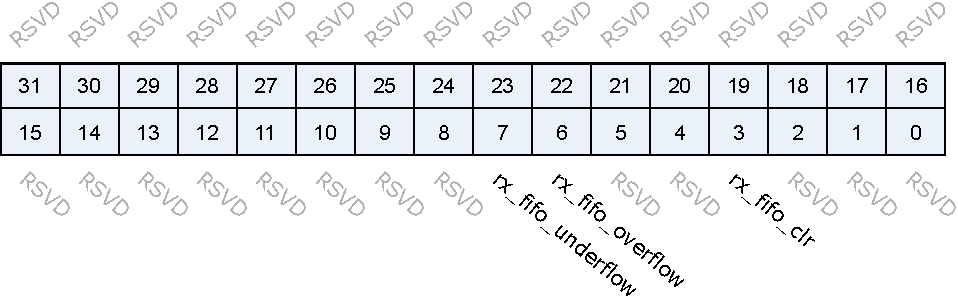
\includegraphics{ir_ir_fifo_config_0.pdf}
\end{figure}

\regdes{31:8&RSVD& & & \\\hline
7&rx\_fifo\_underflow&r&1'b0&Underflow flag of RX FIFO, can be cleared by rx\_fifo\_clr\\\hline
6&rx\_fifo\_overflow&r&1'b0&Overflow flag of RX FIFO, can be cleared by rx\_fifo\_clr\\\hline
5:4&RSVD& & & \\\hline
3&rx\_fifo\_clr&w1c&1'b0&Clear signal of RX FIFO\\\hline
2:0&RSVD& & & \\\hline

}
\subsection{ir\_fifo\_config\_1}
\label{ir-ir-fifo-config-1}
Address:0x40010284
 \begin{figure}[H]
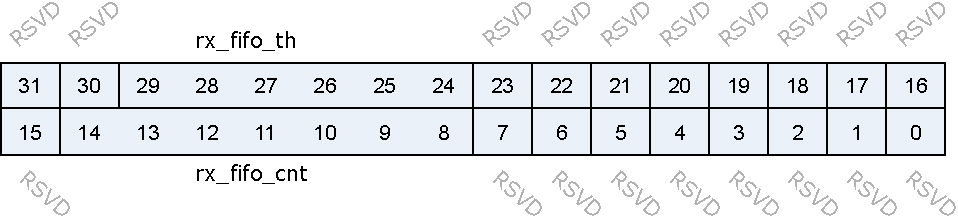
\includegraphics{ir_ir_fifo_config_1.pdf}
\end{figure}

\regdes{31:30&RSVD& & & \\\hline
29:24&rx\_fifo\_th&r/w&6'd0&RX FIFO threshold, irrx\_frdy\_int will not be asserted if rx\_fifo\_cnt is less than this value\\\hline
23:15&RSVD& & & \\\hline
14:8&rx\_fifo\_cnt&r&7'd0&RX FIFO available count\\\hline
7:0&RSVD& & & \\\hline
}

\subsection{ir\_fifo\_rdata}
\label{ir-ir-fifo-rdata}
地址:0x4001028c
 \begin{figure}[H]
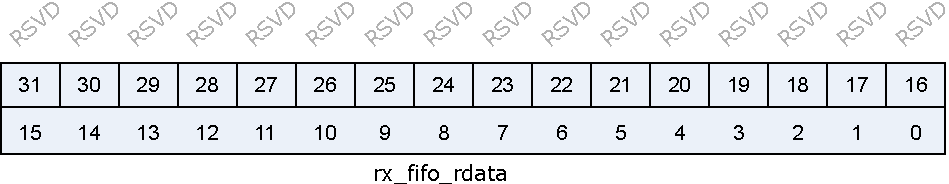
\includegraphics{ir_ir_fifo_rdata.pdf}
\end{figure}

\regdes{31:16&RSVD& & & \\\hline
15:0&rx\_fifo\_rdata&r&16'h0&IRRX FIFO pulse width data for Software Mode\\\hline

}
